\section{Signal Analysis -- simple method (Sachin)}
\label{sec:simple-sachin}

\subsection{Outline}

The simple method of diagnosing sleep apnoea, using audio data from the user's phone that is recorded while he/she is sleeping, was meant to provide a starting point for the development of the app. It served three main purposes:

\begin{itemize}
\item To familiarise us with the typical sleep patterns and with power and frequency content of sleep data
\item As a backup\\
This would give us a method that is able to provide a diagnostic output such as the apnoea-hypopnoea index score from sleep data, even if it was not using machine learning algorithms. 
\item As a point of comparison\\
The simple method would serve as a point of comparison, along with other methods used, with regards to the accuracy of the diagnosis. Using simple metrics such as percentage accuracy of pre-determined apnoea or hypopnoea points in the data against what the model is able to pick out, we can compare the simple model results with our machine learning results. This would allow us to gauge our preformance and also prove that the app is able to diagnose OSA with superior accuracy.
\end{itemize}

MATLAB\textsuperscript{\textregistered{}} was used as the development environment for the simple model. This was due to several reasons. Firstly, our familiarity with MATLAB\textsuperscript{\textregistered{}} from previous projects made it a natural starting point. Secondly, as a dynamically typed language with a user-friendly interface, MATLAB\textsuperscript{\textregistered{}} would enable us to make minor changes to the code and observe the results quicker. Experimentation and tinkering with the code is much easier in MATLAB\textsuperscript{\textregistered{}}  than it is in C/C++ or Java, for example. This ease of experimentation meant that MATLAB\textsuperscript{\textregistered{}} is a good language to start writing the model in, and is used in the initial development of the machine learning HMM model as well. With in-built functions such as audioread, MATLAB\textsuperscript{\textregistered{}}  provided the basic tools with which we could develop the model. Of course, if necessary, the model could later be written in Java for implementation in an Android App - this would be trivial.

The MATLAB\textsuperscript{\textregistered{}} code for the simple model is presented in Appendix \ref{ch:simpleCode}, with detailed explanations. A brief summary is as follows: three \verb!.m! files are created -- \verb!simple.m!, the main script which is run once an audio file is created and stored, and two functions \verb!detectApnea! and \verb!detectApneaVar!, that take a vector of the signal power and a few other parameters as inputs. The \verb!simple.m! script uses the \verb!wavread! or \verb!audioread! function (the user's audio sleep data is recorded in \verb!.wav! format) to read the file and produce a matrix of the audio level values. This is sampled at a lower frequency in order to reduce memory storage. The frequency content of the signal is calculated using the fast fourier transform function (FFT). Along with a plot of the signal, a plot of the frequency content is generated (this is done purely for the programmer's convenience and analysis). The power content is calculated from the signal vector and is used in the \verb!detectApnea! function. An additional function, \verb!detectApneaVar!, is included in the code below highlighting two different ways of analysing the data. The first way, used in \verb!detectApnea!, uses a simple threshold parameter, and searches the signal power vector for prolonged periods of time when the value is below a threshold level. These periods represent apnoeatic episodes when the user's airflow experiences blockages. The second way, used in \verb!detectApneaVar!, aims to identify the sudden inspiration that accompanies the body attempting to re-establish airflow. This is usually characterised by a snorting noise from the user. Instead of simply looking at the power values and comparing them to a threshold, \verb!detectApneaVar! identifes periods of high variance in the signal, which represent the user being `shocked' to start breathing again.

Now, we describe the \verb!simple.m! script in Appendix \ref{sec:simple}. The first part of the code assumes that the user's sleep data has already been recorded using the microphone and has been stored in a file \verb!signal.wav!. This file is read using the \verb!wavread! function as mentioned, and outputs \verb!YRaw!, a two-column matrix (as \verb!wav! encoding uses two channels) as well as \verb!f!, the sampling frequency which is 44.1 kHz. The length of the audio file in seconds, \verb!TMAX!, is also calculated for later use.

A sampling frequency of 44.1 kHz is unnecessarily large and wasteful for an application such as ours -- the frequency content of a 7-minute sample obtained from YouTube \cite{simplevideo} is shown below. The figure on the left represents the spectral density while that on the right represents the information on a logarithmic scale so as to highlight where the useful information is found. As can be seen, there is no useful information that can be found at frequencies above 5 kHz (the duplicated spectra on the left are a result of sampling at the frequency of 44.1kHz). There is no risk of aliasing occuring even if the audio is sampled at 5 kHz. This is where the scale parameter in line 9 above comes in -- it reduces the size of \verb!YRaw! by sampling the already sampled vector (and also combines the two channels into one by taking the average). 

\begin{figure}[htb]
	\centering
	\subfloat[Amplitude Spectra of Raw Audio File]{%
		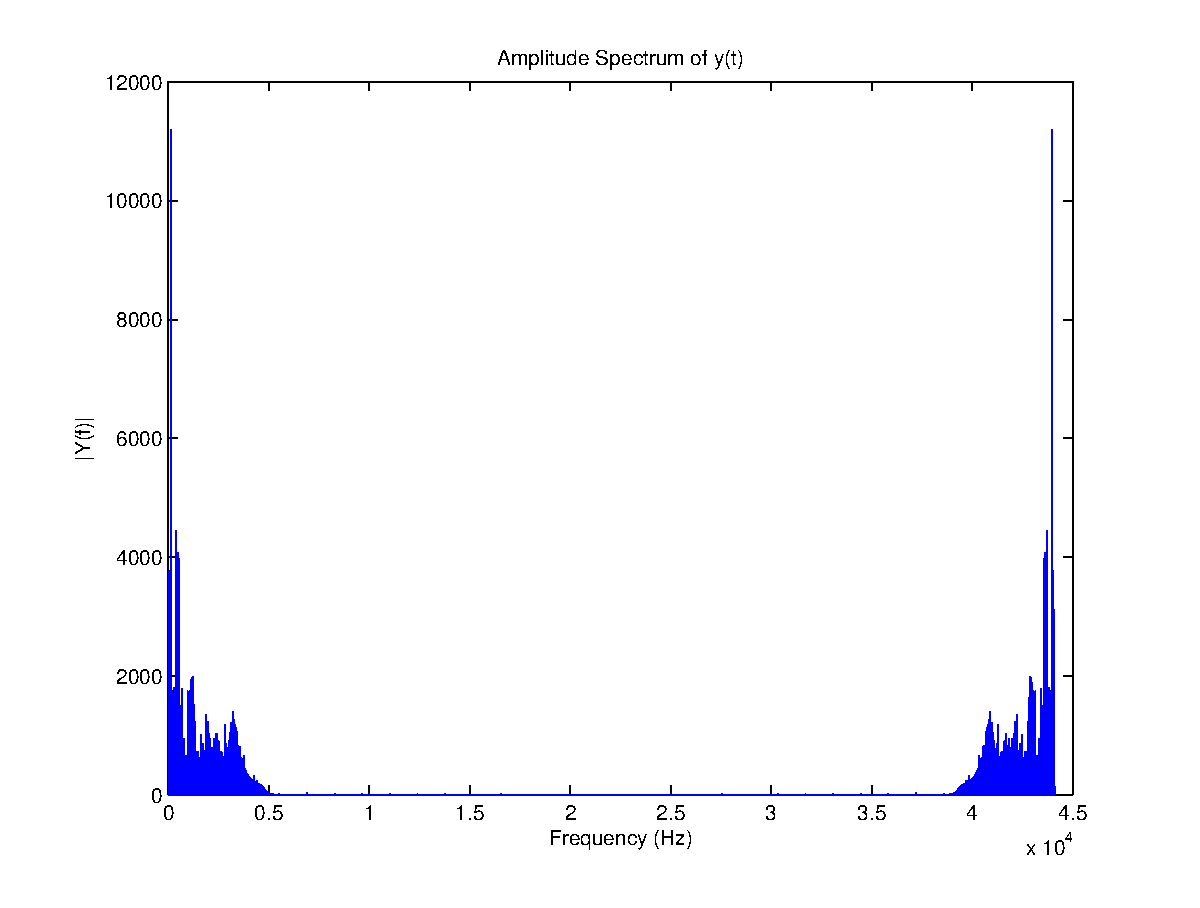
\includegraphics[width=.5\textwidth]{drawings/YRawFreq}}
	\subfloat[Periodogram of Raw Audio File]{%
		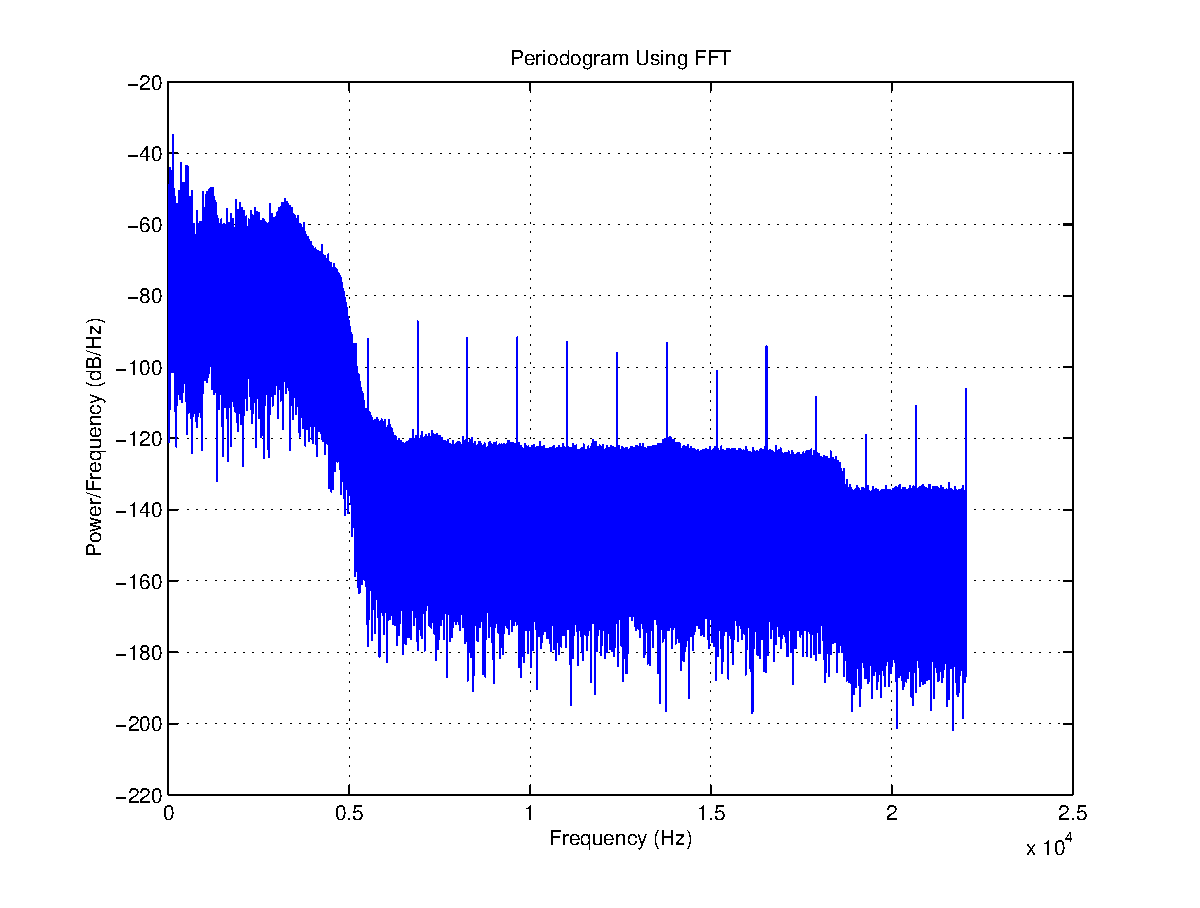
\includegraphics[width=.5\textwidth]{drawings/YRawPeriodogram}}
	\caption{Frequency content of Raw Audio File}
	\label{fig:simpleRawFreqContent}
\end{figure}

The frequency content shown above is calculated using the fast fourier transform (FFT) function in MATLAB\textsuperscript{\textregistered{}}. The function calculates the discrete fourier transform (DFT) of a vector $\vec x = \{x_1, x_2, \dotsc, x_{N}\}$ and returns output $\vec X = \{X_1, X_2, \dotsc, X_{N}\}$  such that
\begin{equation}
X(k) = \sum_{j=1}^{j=N}x(j)\omega^{(j-1)(k-1)}_N
\end{equation}

where

\begin{equation}
\omega_N = e^{(-2\pi i )/N}
\end{equation}

The next few lines of \verb!simple.m! serve to calculate and plot, again, the frequency of the reduced vector \verb!Y! (the figures above are for \verb!YRaw!). The vector power is also created to hold values for the power of the signal at each time period, and will be used in the functions \verb!detectApnea! and \verb!detectApneaVar!.

The next part of the script sets some parameters and uses \verb!detectApnea! as well as \verb!detectApneaVar! to analyse the signal power. The results are then put together and plotted for the programmer's benefit. (The code for doing so is not shown here as it is relatively straightforward and unimportant).

The function \verb!detectApnea! takes as inputs the vector power, the length of the audio file \verb!TMAX!, and parameters \verb!sensitivityMean! and \verb!interval!.

We now describe the code for \verb!detectApnea! shown in Appendix \ref{sec:detectApnea}. Taking inputs \verb!sensitivityMean! and \verb!interval!, \verb!detectApnea! runs through the vector power and identifies when the signal power is below a threshold level for at least a certain interval. This threshold level can be adjusted by changing \verb!sensitivityMean!, and also is affected by the mean value of the overall signal power. This is important, as it is a first step towards ensuring that variations due to users putting the phone further away, which would reduce the overall power of the signal, are taken care of to some extent. The output vector apnoea contains ones and zeroes at every sample point, with ones representing apnoea or hypopnoea episodes.

We now describe the code for \verb!detectApneaVar! shown in Appendix \ref{sec:detectApneaVar}. Instead of simply searching the vector power for values lower than a threshold, \verb!detectApneaVar! attempts to identify periods when there is a sudden spike in the signal power, which means the user has snorted and been shocked into breathing again. Similar to \verb!detectApnea!, \verb!detectApneaVar! uses parameters such as \verb!sensitivityVar! and \verb!windowSize!.

As can be seen, a variance method is used to detect sudden spikes in the signal. A moving window is created of size \verb!windowSize! and is used to temporarily house parts of the vector power. The variance of the values in the window is calculated and if it exceeds a value \verb!maxVariance!, the user is recognised as having had an apnoeatic episode. The window moves on to the immediate next period after updating the output vector \verb!apnea!, and by the end the vector \verb!apnea! contains ones and zeros identifying points in the signal where apnoea is thought to have occurred. Once again, variations due to different users and settings have been accounted for to a certain extent by calculating the value of \verb!maxVariance! from the variance of the entire signal.

The results from the two methods of detecting apnoea are combined together, and the results are plotted below for the sample YouTube video. Firstly, the plot of the power signal, with peaks at regular intervals, confirms that the user has OSA and experiences apnoea and hypopnoea in predictable cycles. The results from the two methods are plotted below the power signal, and exhibit enough correlation such that combining the methods can be justfied. 

\begin{figure}[htb]
\centering
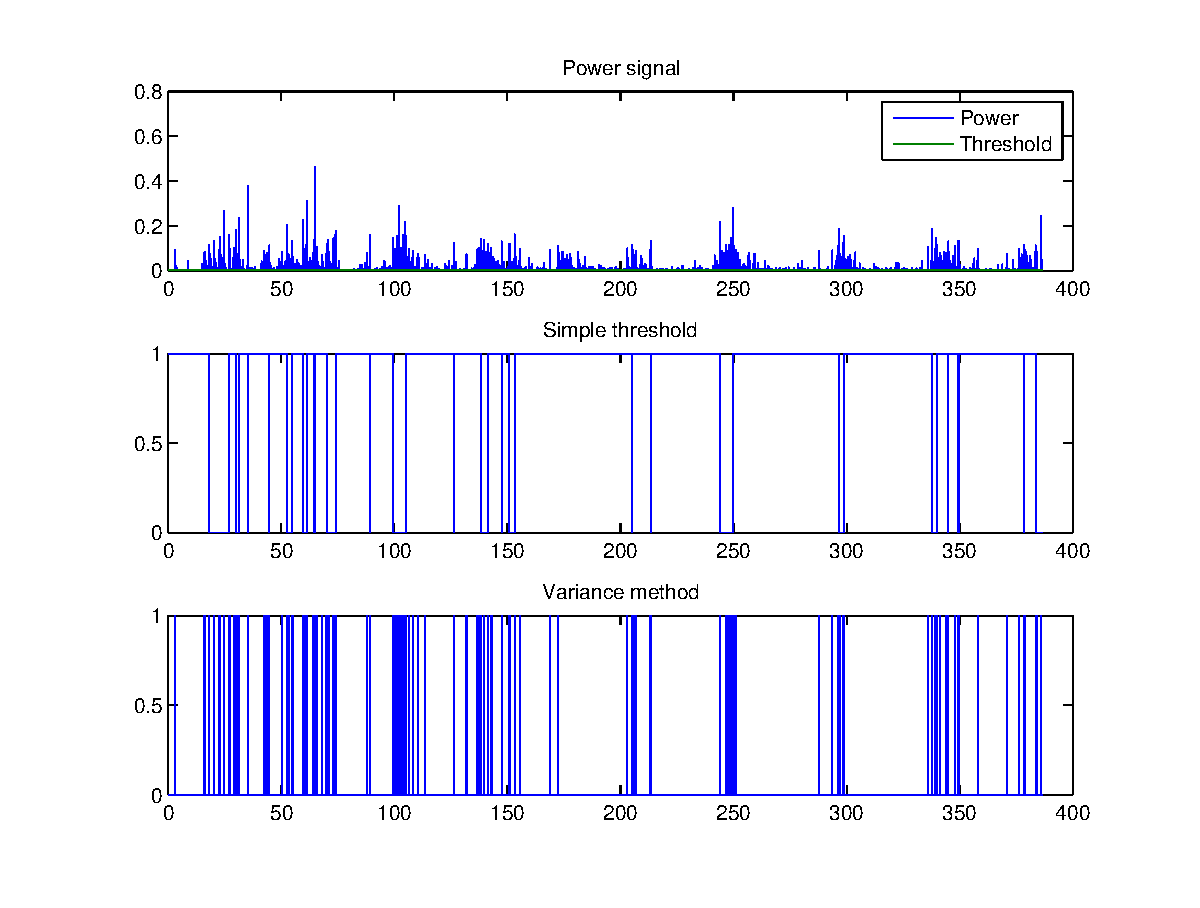
\includegraphics[width=1\textwidth]{drawings/simpleResults}
\caption{Diagnosis Results from 7-minute Sample}
\label{fig:simpleResults}
\end{figure}

\subsection{Limitations of model}

While the simple model we have used above gave us a good starting point and will serve as a point of comparison, it has many limitations. Firstly, the choice of parameter values plays a huge role in the accuracy of the diagnosis. Even though some effort at reducing the effect of variations in noise and signal strength has been taken, the choice of sensitivityMean, sensitivityVar, interval and windowSize is still arbitrary to a large extent. This means that while the model works well for the sample above, there is no guarantee of its effectiveness for other audio signals.

This is where machine learning comes in - needing to choose arbitrary parameter values is removed as the program can be designed to learn, with training data, the best values for parameters and update itself accordingly. The parameters do not have to be the same as those above, of course - this would depend on the exact machine learning model being used.

Secondly, the simple model assumes the existence of an audio file that has already been recorded. Given the average sleep time for adults of seven hours, this could lead to memory storage issues in smartphones where the recording is meant to take place. Some form of compression of the data needs to take place even while recording, and this issue is tackled in the following sections of the report.